




\begin{figure*}[t]

\centerline{
%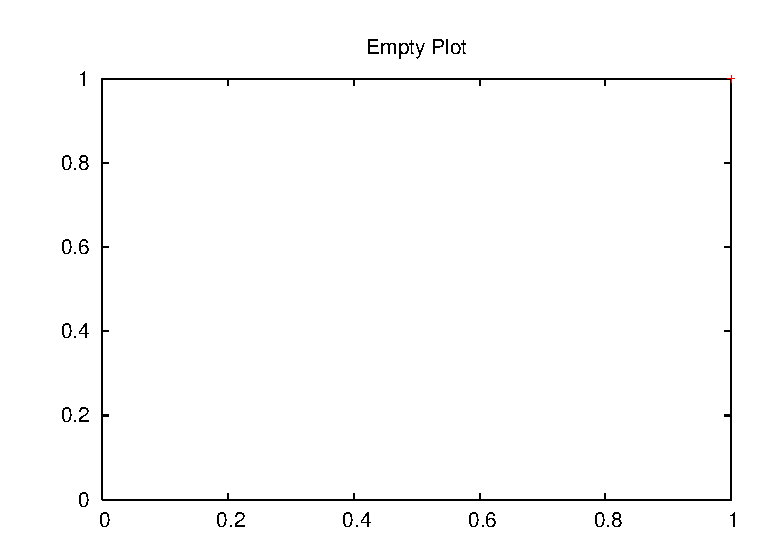
\includegraphics[width=6.5in]{F/empty.eps}
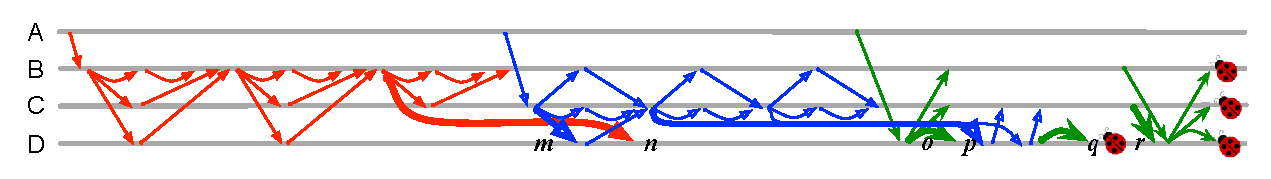
\includegraphics[width=7.0in]{F/paxos/paxos.eps}%
}
\vminfive
\mycaption{fig-paxos}{A Cassandra's Paxos bug}{In \ca{6023}, 
three key-value updates 
(different arrow types)
concurrently execute the Paxos protocol on four nodes
(we simplify from the actual six nodes).
The bug requires three message-message race conditions:
(1) \emph{m} arrives before \emph{n}, 
(2) \emph{o} before \emph{p}, and
(3) \emph{q} before \emph{r}, which collectively
makes D corrupt the data and propagate the corruption
to all replicas after the last broadcast.
Note that the bug would not surface if any of the conditions
did not happen. 
It took us one full day to study this bug.
}
\vten
\end{figure*}

